\documentclass{article}

%Aus dem LaTex Template der Universit�t Stuttgart
%------------------------------------------------
\usepackage[utf8]{inputenc}
\usepackage[T1]{fontenc}
\usepackage[sfdefault]{ClearSans} %% option 'sfdefault' activates Clear Sans as the default text font
\usepackage{cmap}
\usepackage[ngerman]{babel}
\usepackage{graphicx}
\usepackage[pdftex,hyperref,dvipsnames]{xcolor}
\usepackage{listings}
\usepackage[a4paper,lmargin={2cm},rmargin={2cm},tmargin={3.5cm},bmargin = {2.5cm},headheight = {4cm}]{geometry}
\usepackage{amsmath,amssymb,amstext,amsthm}
\usepackage[lined,algonl,boxed]{algorithm2e}
\usepackage{tikz}
\usepackage{hyperref}
\usepackage{url}
\usepackage[inline]{enumitem} % Erm�glicht �ndern der enum Item Zahlen
\usepackage[headsepline]{scrpage2} 
\usepackage{algorithmic} % F�r Pseudocode
\usepackage{ marvosym } % f�r Pfeil(e)
\usepackage{booktabs} % F�r die sch�neren Booktabs-Tabellen
\usepackage{tikz}
\usepackage{pdfpages}
\usepackage{blindtext}
\usepackage{scrextend}
\usepackage{pdfpages}
\usepackage{natbib} % Yannis hat das importiert; TODO: nachfragen, zu was das gut ist
\pagestyle{scrheadings} 
\usetikzlibrary{automata,positioning}


\begin{document}
	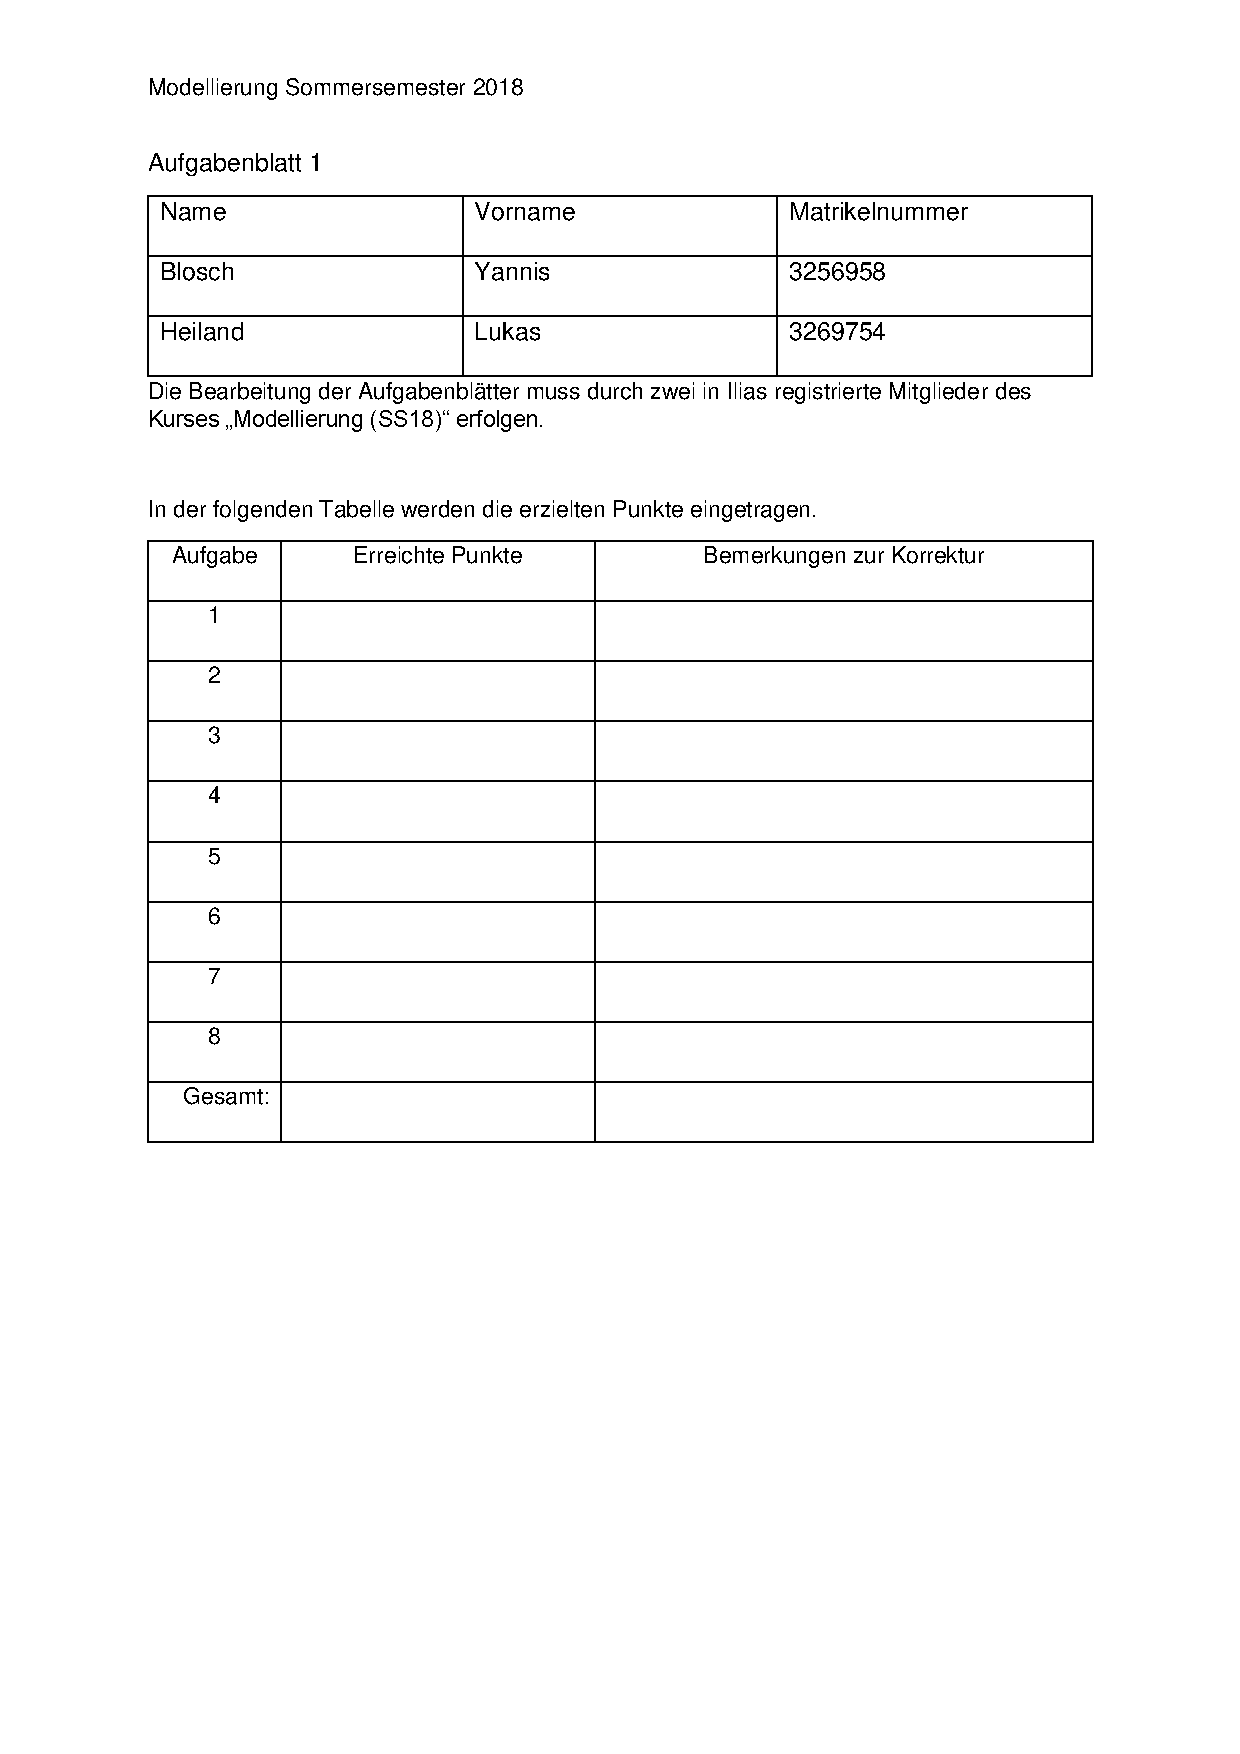
\includepdf[pages=-]{deckblatt.pdf}
	
	% Counter für das Blatt und die Aufgabennummer.
% Ersetze die Nummer des Übungsblattes und die Nummer der Aufgabe
% den Anforderungen entsprechend.
% Beachte:
% \setcounter{countername}{number}: Legt den Wert des Counters fest
% \stepcounter{countername}: Erhöht den Wert des Counters um 1.
\newcounter{sheetnr}
\setcounter{sheetnr}{1} % Nummer des Übungsblattes
\newcounter{exnum}
\setcounter{exnum}{1} % Nummer der Aufgabe

% Befehl für die Aufgabentitel
\newcommand{\exercise}[1]{\section*{Aufgabe \theexnum\stepcounter{exnum} #1}} % Befehl für Aufgabentitel

% Formatierung der Kopfzeile
% \ohead: Setzt rechten Teil der Kopfzeile mit
% Namen und Matrikelnummern aller Bearbeiter
\ohead{Yannis Blosch (3256958)\\
Lukas Heiland (3269754)}
% \chead{} kann mittleren Kopfzeilen Teil sezten
% \ihead: Setzt linken Teil der Kopfzeile mit
% Modulnamen, Semester und Übungsblattnummer
\ihead{Modellierung\\
Sommersemester 2018\\
Blatt \thesheetnr}
	
	\section*{Aufgabe 8.1}.
		\begin{center}
	
			\begin{figure}
				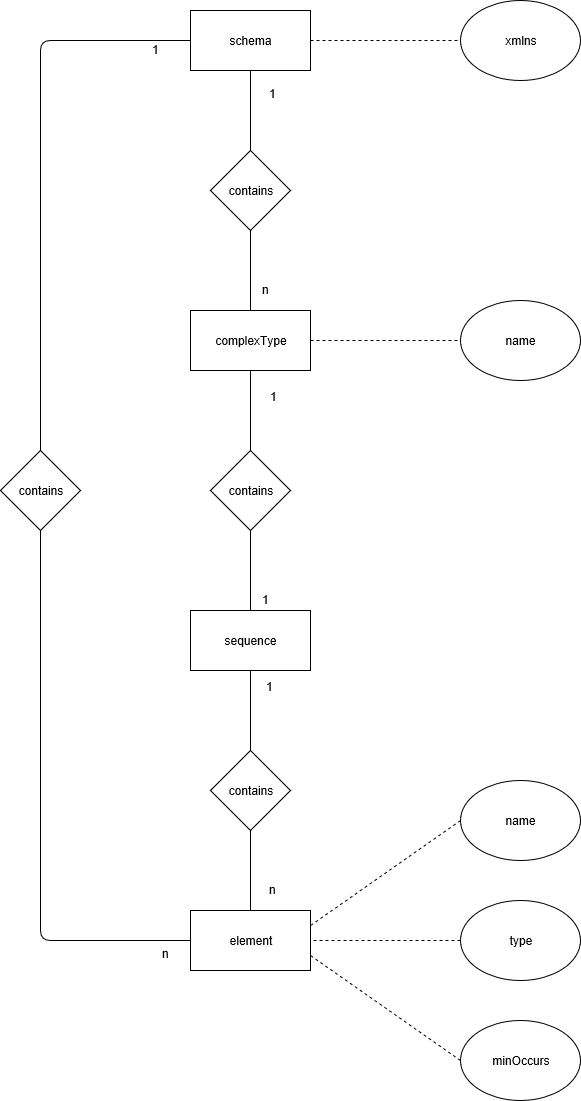
\includegraphics[width=0.4\linewidth]{exercise_8_1.png}
				\caption{Aufgabe 1}
				\label{fig:exercise_8_1.png}
			\end{figure}
		\end{center}
		
		
	\newpage	
	\section*{Aufgabe 8.2}
	\begin{table}[]
		\begin{tabular}{|l|l|lll}
			\cline{1-2}
			Meta-Meta Modell & Backus-Naur Form                &  &  &  \\ \cline{1-2}
			Meta-Modell      & Java Grammatik in BNF           &  &  &  \\ \cline{1-2}
			Modell           & Java Klasse, Programm Code      &  &  &  \\ \cline{1-2}
			Daten            & Programmausführung, Java Objekt &  &  &  \\ \cline{1-2}
		\end{tabular}
	\end{table}
	
	
	\newpage	
	\section*{Aufgabe 8.3}
		\subsection*{a)}
			\begin{figure}
				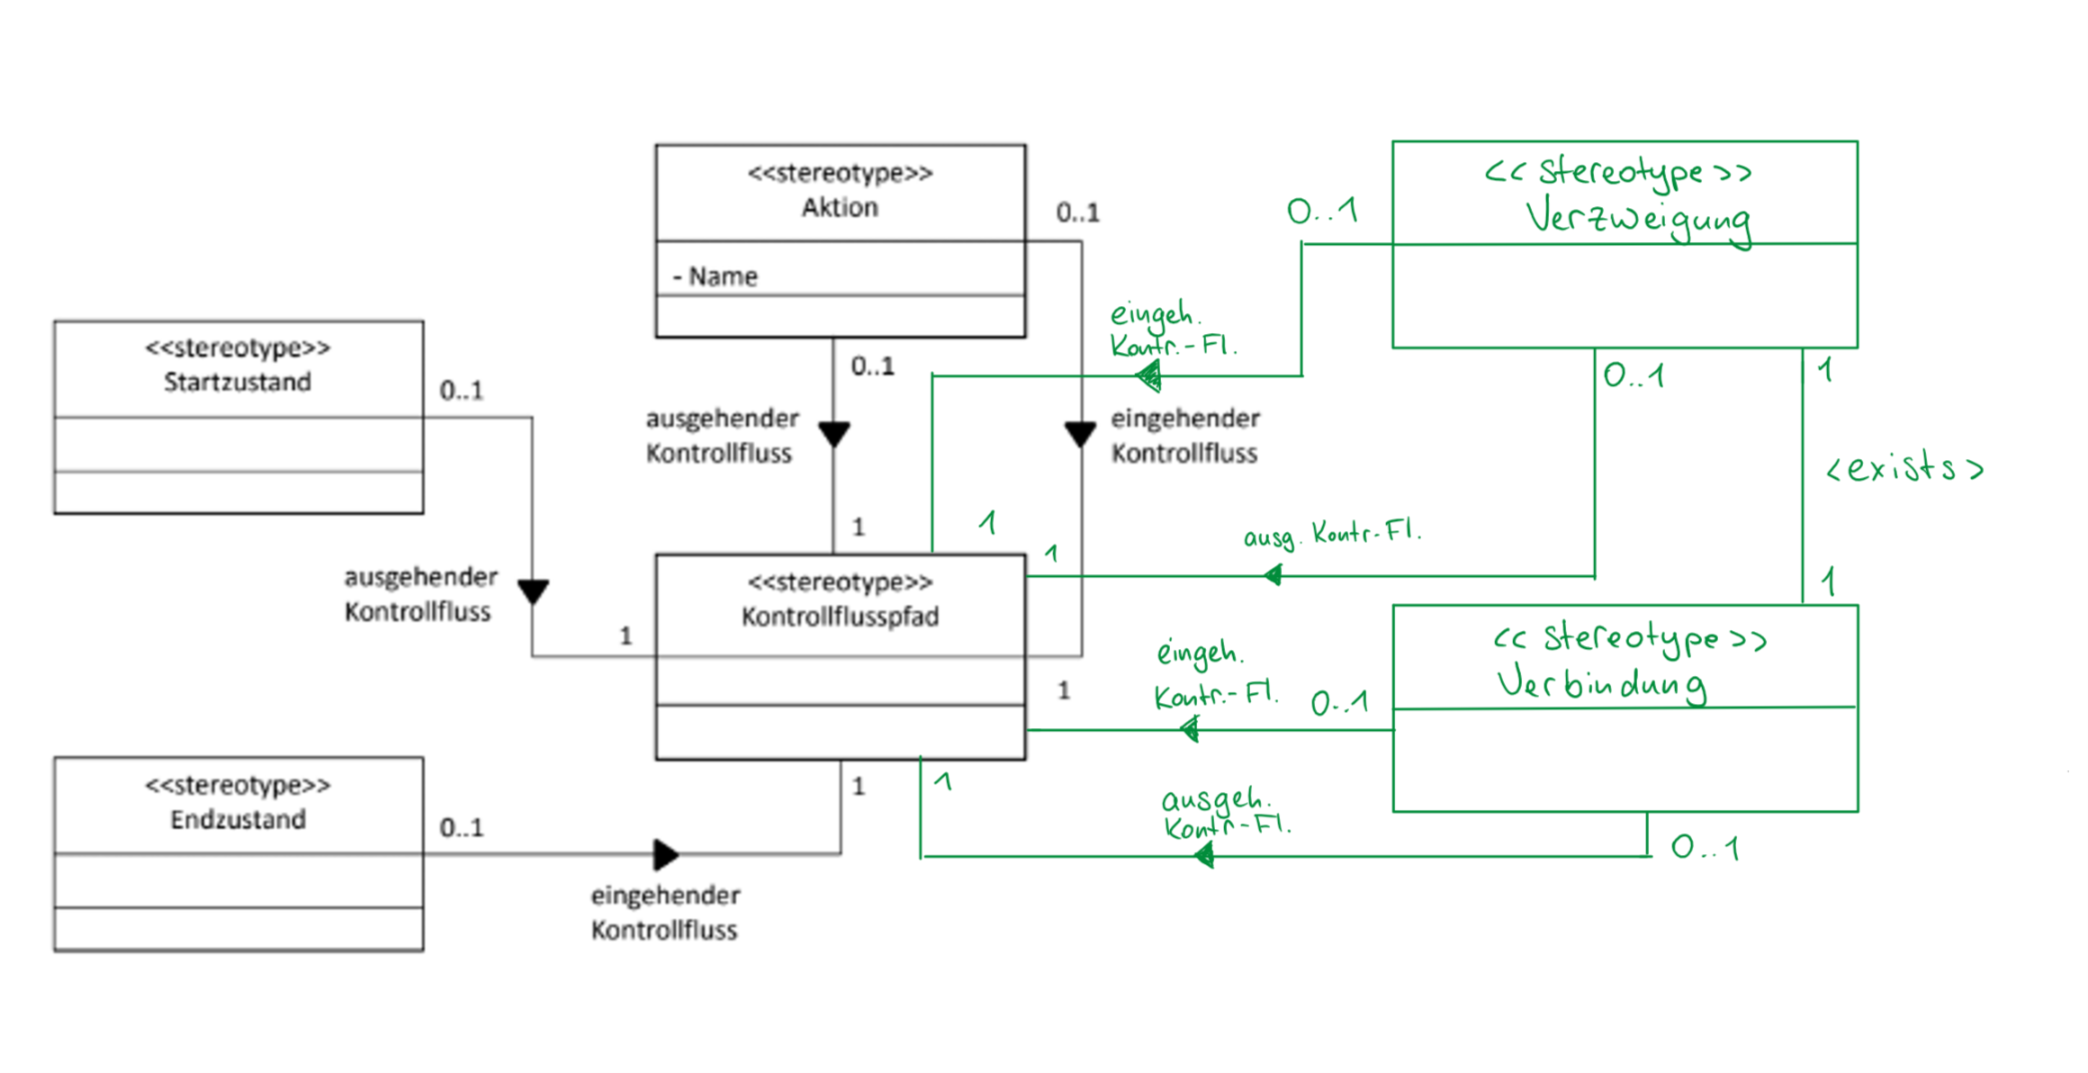
\includegraphics[width=\linewidth]{exercise_8_3_a.png}
%				\caption{Aufgabe 3 a)}
				\label{fig:exercise_8_3_a.png}
			\end{figure}
		
		
		
		\newpage
		\subsection*{b)}
			\begin{figure}
				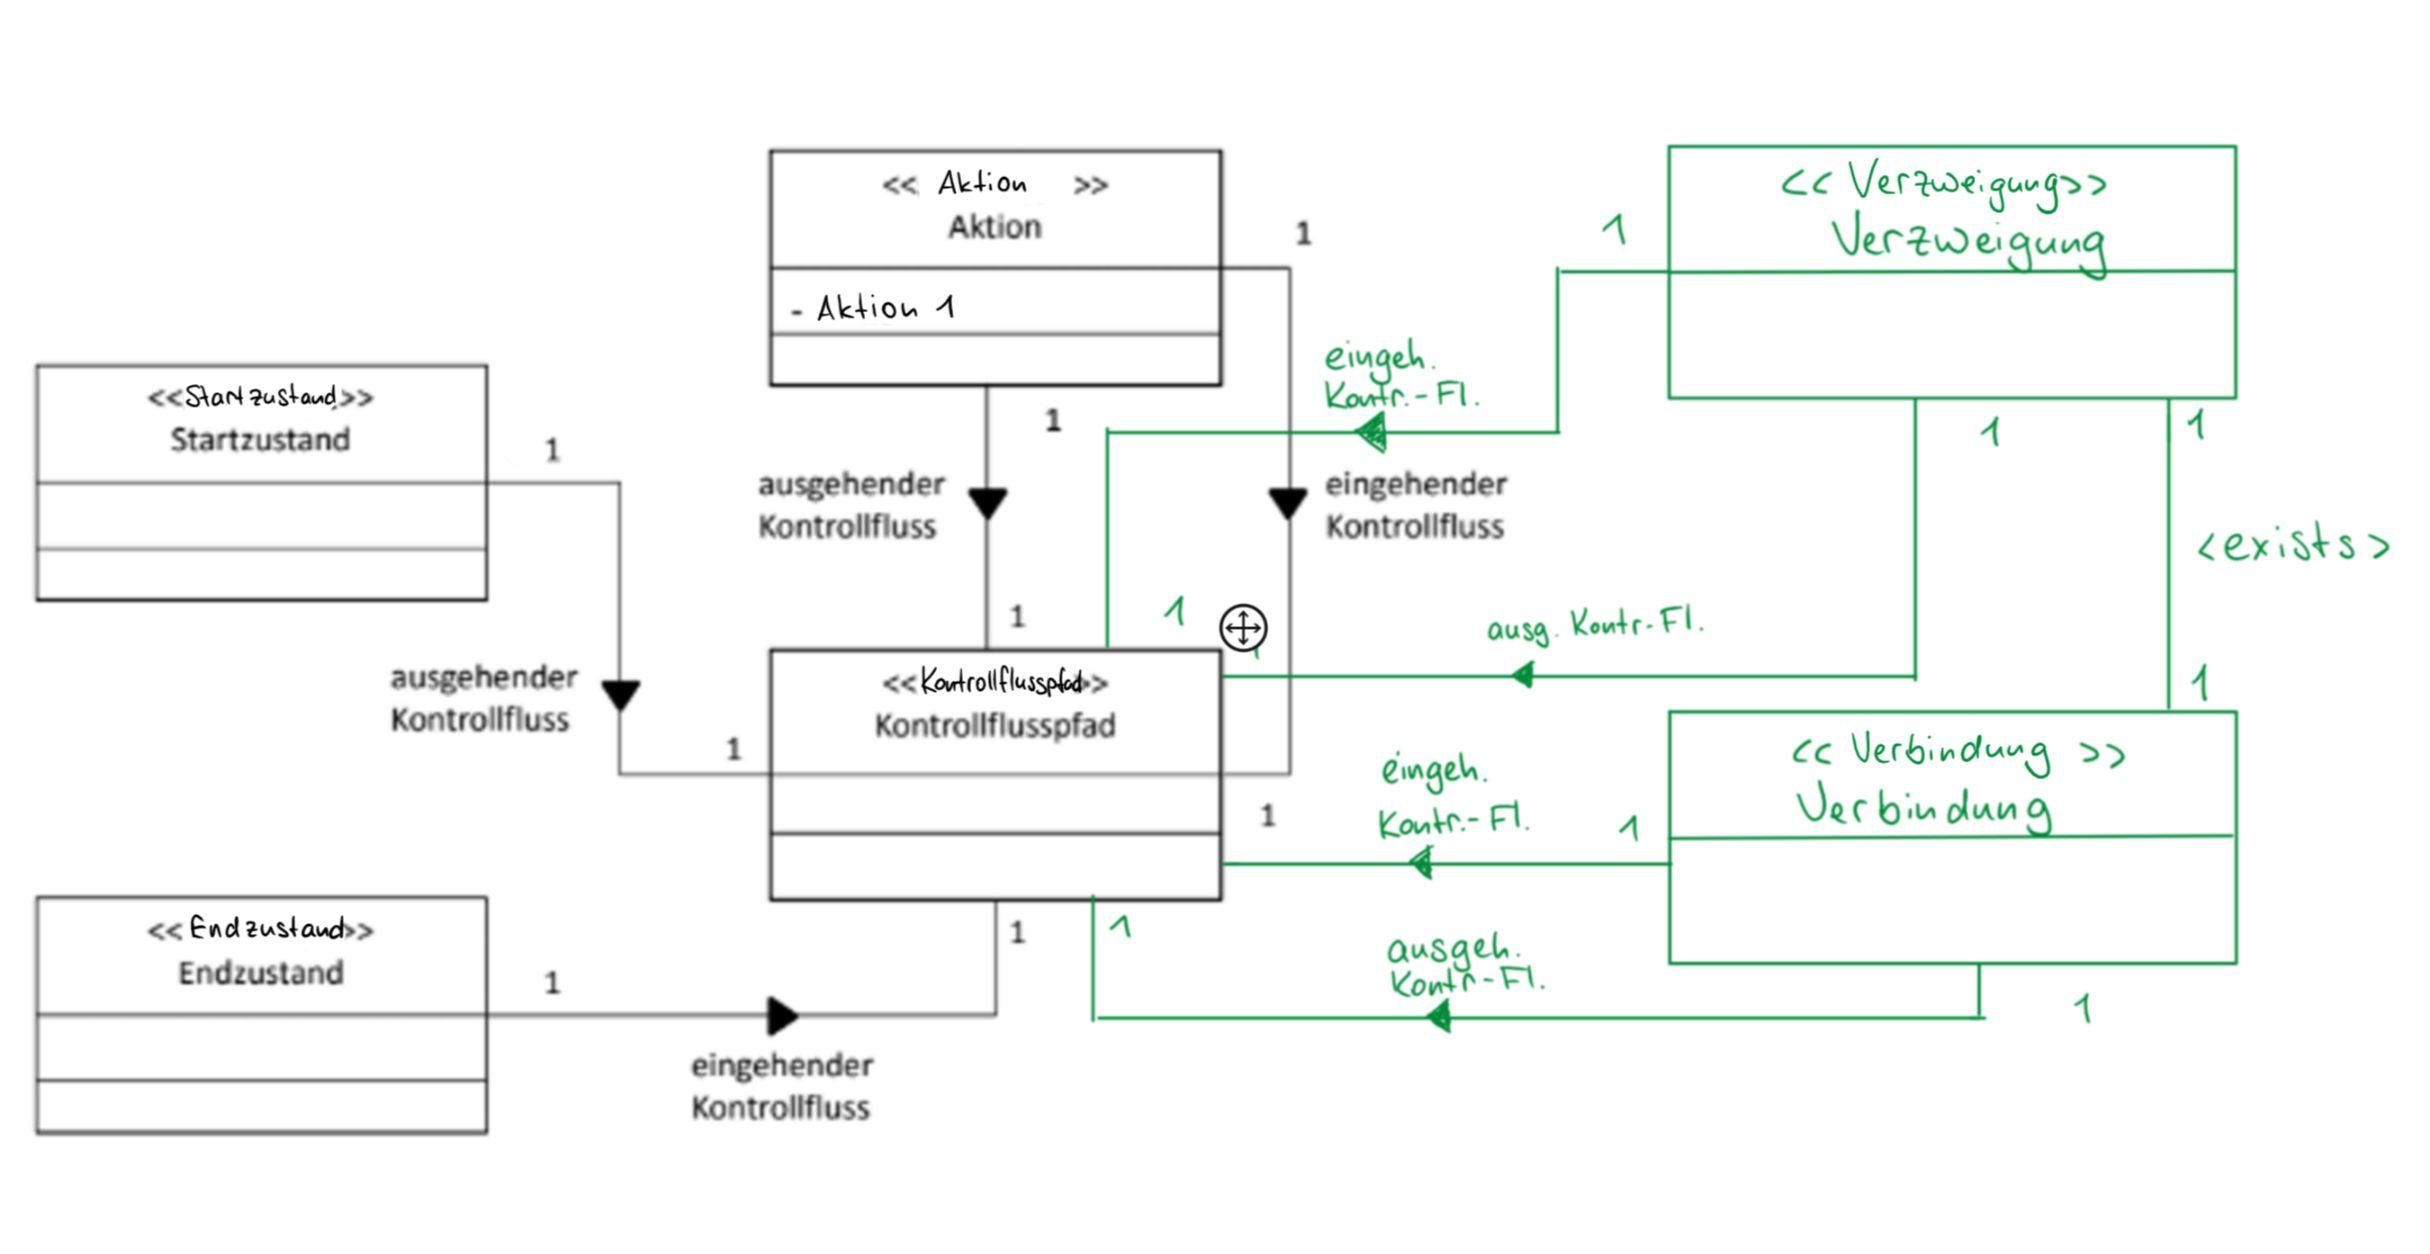
\includegraphics[width=\linewidth]{exercise_8_3_b.png}
				\caption{Aufgabe 3 b)}
				\label{fig:exercise_8_3_b.png}
			\end{figure}
		
\end{document}